% We need layers to draw the block diagram
\begin{figure}[ht]
\centering %

\tikzstyle{block} = [draw,rectangle,thick,minimum height=2em,minimum width=2em]
\tikzstyle{bigblock} = [draw,rectangle,thick,minimum height=2em,minimum width=3em]
\tikzstyle{sum} = [draw,circle,inner sep=0mm,minimum size=2mm]
\tikzstyle{connector} = [->,thick]
\tikzstyle{line} = [thick]	

\tikzstyle{branch} = [circle,inner sep=0pt,minimum size=1mm,fill=black,draw=black]
\tikzstyle{guide} = []

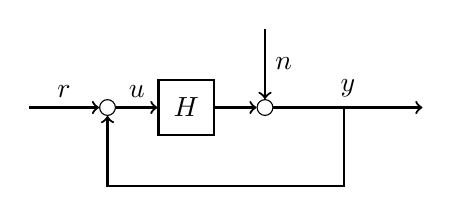
\begin{tikzpicture}[scale=1, auto]

    %  Loop function
    \node[coordinate]												(input) 		{};
		\node[sum,right of=input]		(u)	{};
		\node[block,right of =u] 			(H) 					{$H$};
		\node[sum,right of=H]				(sumn)			{};
		\node[coordinate,above of=sumn]				(n)			{};
		\node[coordinate,right of =sumn]				(y) 					{$\mathbf{H}$};
		\node[coordinate,right of =y]				(output) 				{};
		
		\node[coordinate,below of = y] (yfb) {};
		\node[coordinate,below of = u] (sumu) {};
		
		% Draw connectors
		\draw[connector] (input) -- node {$r$} (u);
				\draw[connector] (u) -- node {$u$} (H);
		\draw[connector] (H) -- node {} (sumn);
				\draw[connector] (sumn) -- node {$y$} (output);
		\draw[connector] (n) -- node {$n$} (sumn);	
		
		\draw[connector] (y) -- (yfb) -- (sumu) -- (u);

    \end{tikzpicture}
		
		\end{figure}